%---------- Inleiding ---------------------------------------------------------

\section{Introductie}%
\label{sec:introductie}

Het alledaagse gebruik van mobiele toetsenborden op Android-apparaten onderstreept hun cruciale rol in ons dagelijks leven. Hoewel deze toetsenborden zich hoofdzakelijk richten op nauwkeurige spelling- \& grammatica\-controle, blijft de bescherming van privacy voornamelijk een verantwoordelijkheid van de ontwikkelaars.

Dit onderzoek beoogt een machtswisseling, door niet alleen privacy te waarborgen, maar ook de controle terug te geven aan de consument. Het doel is een privacybewust spelling- \& grammatica\-controle-toetsenbord voor Android ontwikkelen, met een initiële focus op het Nederlands, mogelijk gebruikmakend van RobBERT, een Nederlandstalige variant van BERT (Bidirectional Encoder Representations from Transformers) ~\autocite{Delobelle2020} .

Binnen het bredere spectrum van privacybewuste informatieverwerking fungeert dit onderzoek als katalysator om privacy terug te brengen in handen van de eindgebruiker. Gebruikers omvat iedereen met een Android-toestel, met een initiële focus op het Nederlands, vooral voor degenen die extra zorg dragen voor hun data.

Hoewel toetsenbord ontwikkelaars belang he\-ch\-ten aan privacy, blijft de controle over gebruikersgegevens momenteel gecentraliseerd ~\autocite{GrammarlyInc2023, SECL2023}. Dit roept de vraag op hoe een privacybewust spel\-ling- \& grammatica\-controle-toetsenbord kan ontwikkelt worden dat niet alleen nauwkeurig is, maar ook offline gebruikt kan worden. Hierdoor behouden gebruikers volledige controle over hun data.

In het licht van deze uitdaging, omvat dit onderzoek de volgende kernvragen:

\begin{enumerate}
    \item Welke taalproblemen kunnen worden gecorrigeerd met technologieën zoals BERT, RobBERT en RobBERTje?
    \item Hoe kan een dergelijk toetsenbord worden ontworpen om initieel de Nederlandse taal te ondersteunen met de flexibiliteit voor uitbreiding naar andere talen?
    \item Op welke wijze kan dit toetsenbord aangepast worden voor diverse gebruikssituaties buiten de initiële implementatie?
    \item Wat is de ideale evenwicht tussen nauwkeurigheid en privacy in de ontwikkeling van dit toetsenbord?
    \item Hoe kan de gebruiker de controle over zijn of haar persoonlijke data behouden?
    \item Wat zijn de gevolgen voor de prestaties van het toetsenbord bij de integratie van spelling- en grammaticacontrole?
    \item Is de beoogde oplossing voldoende schaalbaar om meerdere talen en uitgebreide gebruikssituaties te ondersteunen?
    \item Welke technische uitdagingen moeten worden overwonnen om hoge prestaties en sch\-aal\-baar\-heid te garanderen?
\end{enumerate}


Dit onderzoek beoogt niet alleen de ontwikkeling van een privacybewust spel\-ling- \& grammatica\-controle-toetsenbord voor Android, maar ook de integratie van een lokale Natural Language Processing (NLP) engine. Deze benadering stelt gebruikers in staat om het toetsenbord offline te gebruiken, waardoor ze volledige controle hebben over hun gegevens. Bij succesvolle prototypen wordt er gestreefd naar uitbreiding over verschillende talen \& casussen, met een blijvende focus op privacy \& gebruikersautonomie. Het uiteindelijke doel is niet alleen een werkend prototype maar ook de versterking van gebruikers in termen van privacy \& controle over hun eigen gegevens.

%---------- Stand van zaken ---------------------------------------------------

\section{State-of-the-art}%
\label{sec:state-of-the-art}

\subsection{Natural Language Processing}
Natural Language Processing (NLP) is een tak van machine learning die computers de capaciteit geeft om menselijke taal te interpreteren, manipuleren en begrijpen. In de hedendaagse samenleving verzamelen organisaties aanzienlijke hoeveelheden spraak- en tekstgegevens uit diverse communicatiekanalen zoals e-mails, tekstberichten, sociale media-feeds, video's, audio-op\-na\-mes, en meer. NLP-software wordt ingezet om deze gegevens automatisch te verwerken, de intentie of sentiment in de boodschap te analyseren, en in real-time te reageren op menselijke communicatie ~\autocite{AWSI2023}. 

Wat NLP bijzonder relevant maakt voor het privacyprobleem is de mogelijkheid om deze technologie lokaal te implementeren. In plaats van afhankelijk te zijn van externe servers voor gegevensverwerking, kan een lokaal NLP-systeem draaien op het Android-apparaat zelf. Dit betekent dat de gevoelige tekstgegevens van de gebruiker niet extern worden verzonden voor verwerking, wat de controle over persoonlijke data vergroot en pri\-va\-cy\-risico's ver\-min\-dert ~\autocite{Cistac2019}.

Het integreren van een lokale NLP-engine in het spelling- en grammaticacontrole-toetsenbord voor Android biedt daarom niet alleen voordelen op het gebied van privacy, maar ook een praktische manier om gegevens lokaal te verwerken zonder afbreuk te doen aan de nauwkeurigheid en functionaliteit van de taalverwerking.

\subsection{BERT, RobBERT, RobBERTje}
De recente vooruitgang in taalmodellen heeft geleid tot opmerkelijke prestaties, waarbij BERT (Bidirectional Encoder Representations from Tran\-s\-for\-mers) een prominente rol speelt. Deze modellen hebben substantiële verbeteringen opgeleverd voor diverse natuurlijke taaltaken, maar hun implementatie en fine-tuning vereisen aanzienlijke computermiddelen vanwege het grote aantal parameters ~\autocite{Delobelle2020}.

Voor de Nederlandse taal heeft RobBERT zich onderscheiden als een geoptimaliseerde tegenhanger van BERT, gebaseerd op de RoBERTa-be\-na\-de\-ring. Recentelijk zijn gedistilleerde versies van het RobBERT-model geïntroduceerd, ge\-naa\-md RobBERTje. Deze distillaties variëren in het gebruik van distillatiecorpus, inclusief het al dan niet schudden en samenvoegen van opeenvolgende zinnen. ~\autocite{Delobelle2021}

Vergelijkend onderzoek tussen distillatiearchitecturen heeft aangetoond dat RobBERTje-mo\-del\-len vergelijkbare prestaties leveren, ongeacht of ze worden getraind met geschudde of niet-geschudde datasets. Bovendien bleek dat het willekeurig samenvoegen van opeenvolgende zinnen resulteerde in modellen die sneller trainen en beter presteren op taken met lange sequenties. De keuze van distillatiearchitectuur bleek ook van invloed te zijn, waarbij de grotere DistilBERT-arch\-i\-tec\-tuur aanzienlijk beter presteerde dan de Bort-hyperparametrisering ~\autocite{Delobelle2021}.

Deze gedistilleerde modellen bieden niet alleen efficiëntere training en lichtgewicht implementatie, maar vertonen ook minder genderstereotype bias dan hun 'leraar'-model. Dit maakt RobBERTje een krachtig pre-trained model voor verschillende Nederlandse taaltaken, met verbeterde resultaten, vooral bij kleinere datasets. ~\autocite{Delobelle2022}

In het bredere spectrum van privacybewuste informatieverwerking kan het gebruik van lokale NLP-engines zoals RobBERTje bijdragen aan de privacy van gebruikers. Door taalverwerking lokaal uit te voeren, worden gevoelige tekstgegevens niet extern verzonden, wat de controle over persoonlijke data vergroot en de privacyrisico's vermindert. Bovendien biedt dit een efficiënte oplossing voor opslag en CPU-intensiteit op mobiele apparaten zoals Android, wat resulteert in een meer geoptimaliseerd gebruik van resources.

Deze technologische ontwikkelingen in de v\-orm van RobBERTje bieden niet alleen verbeteringen in taalverwerking, maar hebben ook implicaties voor privacybewuste toepassingen op mobiele apparaten, waarbij een balans wordt gevonden tussen technische efficiëntie en gebruikersprivacy.

\subsection{Gebruikerservaring \& Optimalisatie}

Letterfrequentie, een belangrijk aspect van t\-oe\-ts\-enbord ontwerp, houdt rekening met de m\-ee\-st voorkomende letters in een taal. Dit principe wordt ook ondersteund door Fitts' Law, die stelt dat frequenter gebruikte toetsen meer schermruimte moeten krijgen. Dergelijke optimalisaties hebben potentie om de snelheid van typen op virtuele toetsenborden te vergroten ~\autocite{Gelormini2013}.

Een andere invalshoek om de gebruikerservaring te verbeteren, richt zich op energie-efficiëntie. Een studie analyseerde de energieprestaties van vijf veelgebruikte virtuele toetsenborden in het Android-ecosysteem. Hierbij werden scenario's onderzocht, zoals het gebruik van woordvoorspelling, en concludeerde dat er aanzienlijke prestatieverschillen zijn tussen verschillende toetsenborden (3). Door het gebruik van de meest efficiënte toetsenbord zou het mogelijk zijn om bijna 18\% energie te besparen op Android-apparaten. ~\autocite{Rua2020}

Het samenvoegen van deze benaderingen - optimalisatie op basis van letterfrequentie, lettervoorspelling, key resizing, en energie-efficiëntie - biedt een breed scala aan strategieën om de gebruikerservaring van virtuele toetsenborden te verbeteren. De integratie van deze technologieën in de context van privacybewuste NLP-engines kan een veelbelovende stap zijn naar meer efficiënte en gebruikersvriendelijke virtuele toetsenborden op Android-apparaten.

\subsection{TensorFlow \& Firebase}

In het kader van een geavanceerd toetsenbord voor Android-apparaten ontwikkelen, speelt TensorFlow een cruciale rol als kerncomponent. Het is een open-source machine learning-bibliotheek, dat een krachtig platform biedt voor het creëren en trainen van machine learning-modellen. Deze modellen worden geoptimaliseerd met TensorFlow Lite, wat essentieel is voor de implementatie op mobiele apparaten. De veelzijdigheid en prestatiegerichtheid van TensorFlow maken het een ideale keuze om geavanceerde spelling- en grammaticacontrole mogelijk te maken op het lokale niveau van het Android-apparaat.

Firebase, als een uitgebreid ontwikkelingsplatform, faciliteert de integratie van TensorFlow-mo\-del\-len in Android-apps. Firebase ML stelt ontwikkelaars in staat om machine learning-func\-tio\-na\-li\-teit rechtstreeks in hun apps te implementeren. Deze integratie met Firebase is van bijzonder belang omdat het lokale implementatie op het Android-apparaat mogelijk maakt, zonder externe serverafhankelijkheden. Dit draagt niet alleen bij aan de efficiëntie van de implementatie, maar waarborgt ook de privacy van gebruikers, aangezien gegevens niet extern worden verwerkt.

Een relevante codelab van \textcite{ulukaya2023} illustreert concreet hoe TensorFlow en Firebase kunnen worden samengevoegd. In dit scenario werden TensorFlow-modellen gekoppeld aan Firebase en vervolgens geïntegreerd in Android-applicaties. Deze integratie benadrukt de mogelijkheid om machine learning-modellen direct op het apparaat te laten draaien, wat niet alleen snelheid en efficiëntie oplevert, maar ook voldoet aan privacyrichtlijnen door gegevensverwerking op het apparaat zelf te houden.

Door gebruik te maken van TensorFlow en Firebase als centrale tools in de ontwikkeling van het toetsenbord, wordt beoogd geavanceerde func\-tio\-na\-li\-teit te bieden, evenals een geoptimaliseerde implementatie die inspeelt op gebruikersbehoeften en privacyvereisten op een Android-apparaat.

%---------- Methodologie ------------------------------------------------------
\section{Methodologie}%
\label{sec:methodologie}

\subsection{Onderzoeksaanpak}

\subsubsection{Voorbereidingsfase}
\begin{itemize}
    \item Identificatie van vereisten: De functionele en niet-functionele vereisten voor het privacybewuste toetsenbord worden vastgesteld, rekening houdend met RobBERTje en privacyrichtlijnen.
    \item Gebruikersverkenning: Polsing naar potentiële gebruikers om een grondig begrip te krijgen van hun behoeften en voorkeuren, met specifieke aandacht voor Android-gebruikers in Nederland die waarde hechten aan privacy.
\end{itemize}

\subsubsection{Ontwerp- en Planning}
\begin{itemize}
    \item Ontwerp van de gebruikersinterface: Lay-out en interactie van het toetsenbord worden uitgewerkt met aandacht voor gebruikerservaring en privacy.
    \item Planning en milestones: Een gedetailleerd ontwikkelingsplan wordt opgesteld met mijlpalen voor implementatie en evaluatie.
\end{itemize}

\subsubsection{Integratie en Implementatie}
\begin{itemize}
    \item Integratie van RobBERTje: De Nederlandstalige BERT-variant, RobBERTje, wordt geïntegreerd als kerncomponent van het toetsenbord.
    \item Ontwikkeling van privacyfuncties: Implementatie van privacybeschermende functies, zoals lokale NLP-verwerking en controle over gebruikersgegevens.
    \item Implementatie van TensorFlow: Gebruik van TensorFlow en TensorFlow Lite voor geavanceerde spelling- en grammaticacontrole.
    \item Firebase-integratie: Implementatie van Firebase voor het inbedden van het TensorFlow-model, wat resulteert in naadloze integratie met de applicatie op Android-apparaten.
    \item Optimalisatie van Implementatie: Bevestiging van efficiënt gebruik van resources, optimalisatie van CPU- en opslaggebruik op Android-apparaten, en privacygerichte implementatie.
\end{itemize}

\subsubsection{Testen en Evaluatie}
\begin{itemize}
    \item Gebruikerstesten: Uitvoeren van tests om functionaliteit, nauwkeurigheid en pri\-va\-cy \linebreak van het toetsenbord te evalueren.
    \item Verbeteringen aanbrengen: Iteratieve aanpassingen aan het toetsenbord op basis van gebruikersfeedback en prestatieresultaten.
\end{itemize}

\subsection{Datacollectie en -analyse}

\subsubsection{Gegevensbronnen}
\begin{itemize}
    \item Verzameling van gebruikersgegevens: Beperkte verzameling van gegevens tot lokale opslag op het Android-apparaat, in overeenstemming met privacyrichtlijnen.
    \item Evaluatiegegevens: Verzameling van gegevens uit gebruikerstesten en prestatie-eva\-lu\-a\-ties.
\end{itemize}

\subsubsection{Analysemethode}
\begin{itemize}
    \item Kwalitatieve analyse van gebruikersfeedback: Beoordeling van gebruikerservaring, voorkeuren en problemen tijdens testen.
    \item Kwantitatieve analyse van prestatiegegevens: Evaluatie van nauwkeurigheid en efficiëntie van lokale NLP-verwerking.
\end{itemize}


Deze methodologie vormt het raamwerk voor de ontwikkeling, implementatie en evaluatie van het privacybewuste toetsenbord, met een focus op nauwkeurigheid, gebruikersprivacy en lokale verwerking van NLP-functionaliteit.


%---------- Verwachte resultaten ----------------------------------------------
\section{Verwacht resultaat, conclusie}%
\label{sec:verwachte_resultaten}

In deze sectie worden de verwachte resultaten van het onderzoek besproken, waarbij grafische voorstellingen anticiperen op mogelijke uitkomsten. Het doel is een heldere visie te geven op de verwachte bijdrage aan het vakgebied en de potentiële meerwaarde voor de doelgroep.

\subsection{Verwachte Resultaten}

\subsubsection{Grafische Voorstelling van NLP-Verwer\-kings\-correctheid}

\begin{figure}[ht]
    \centering
    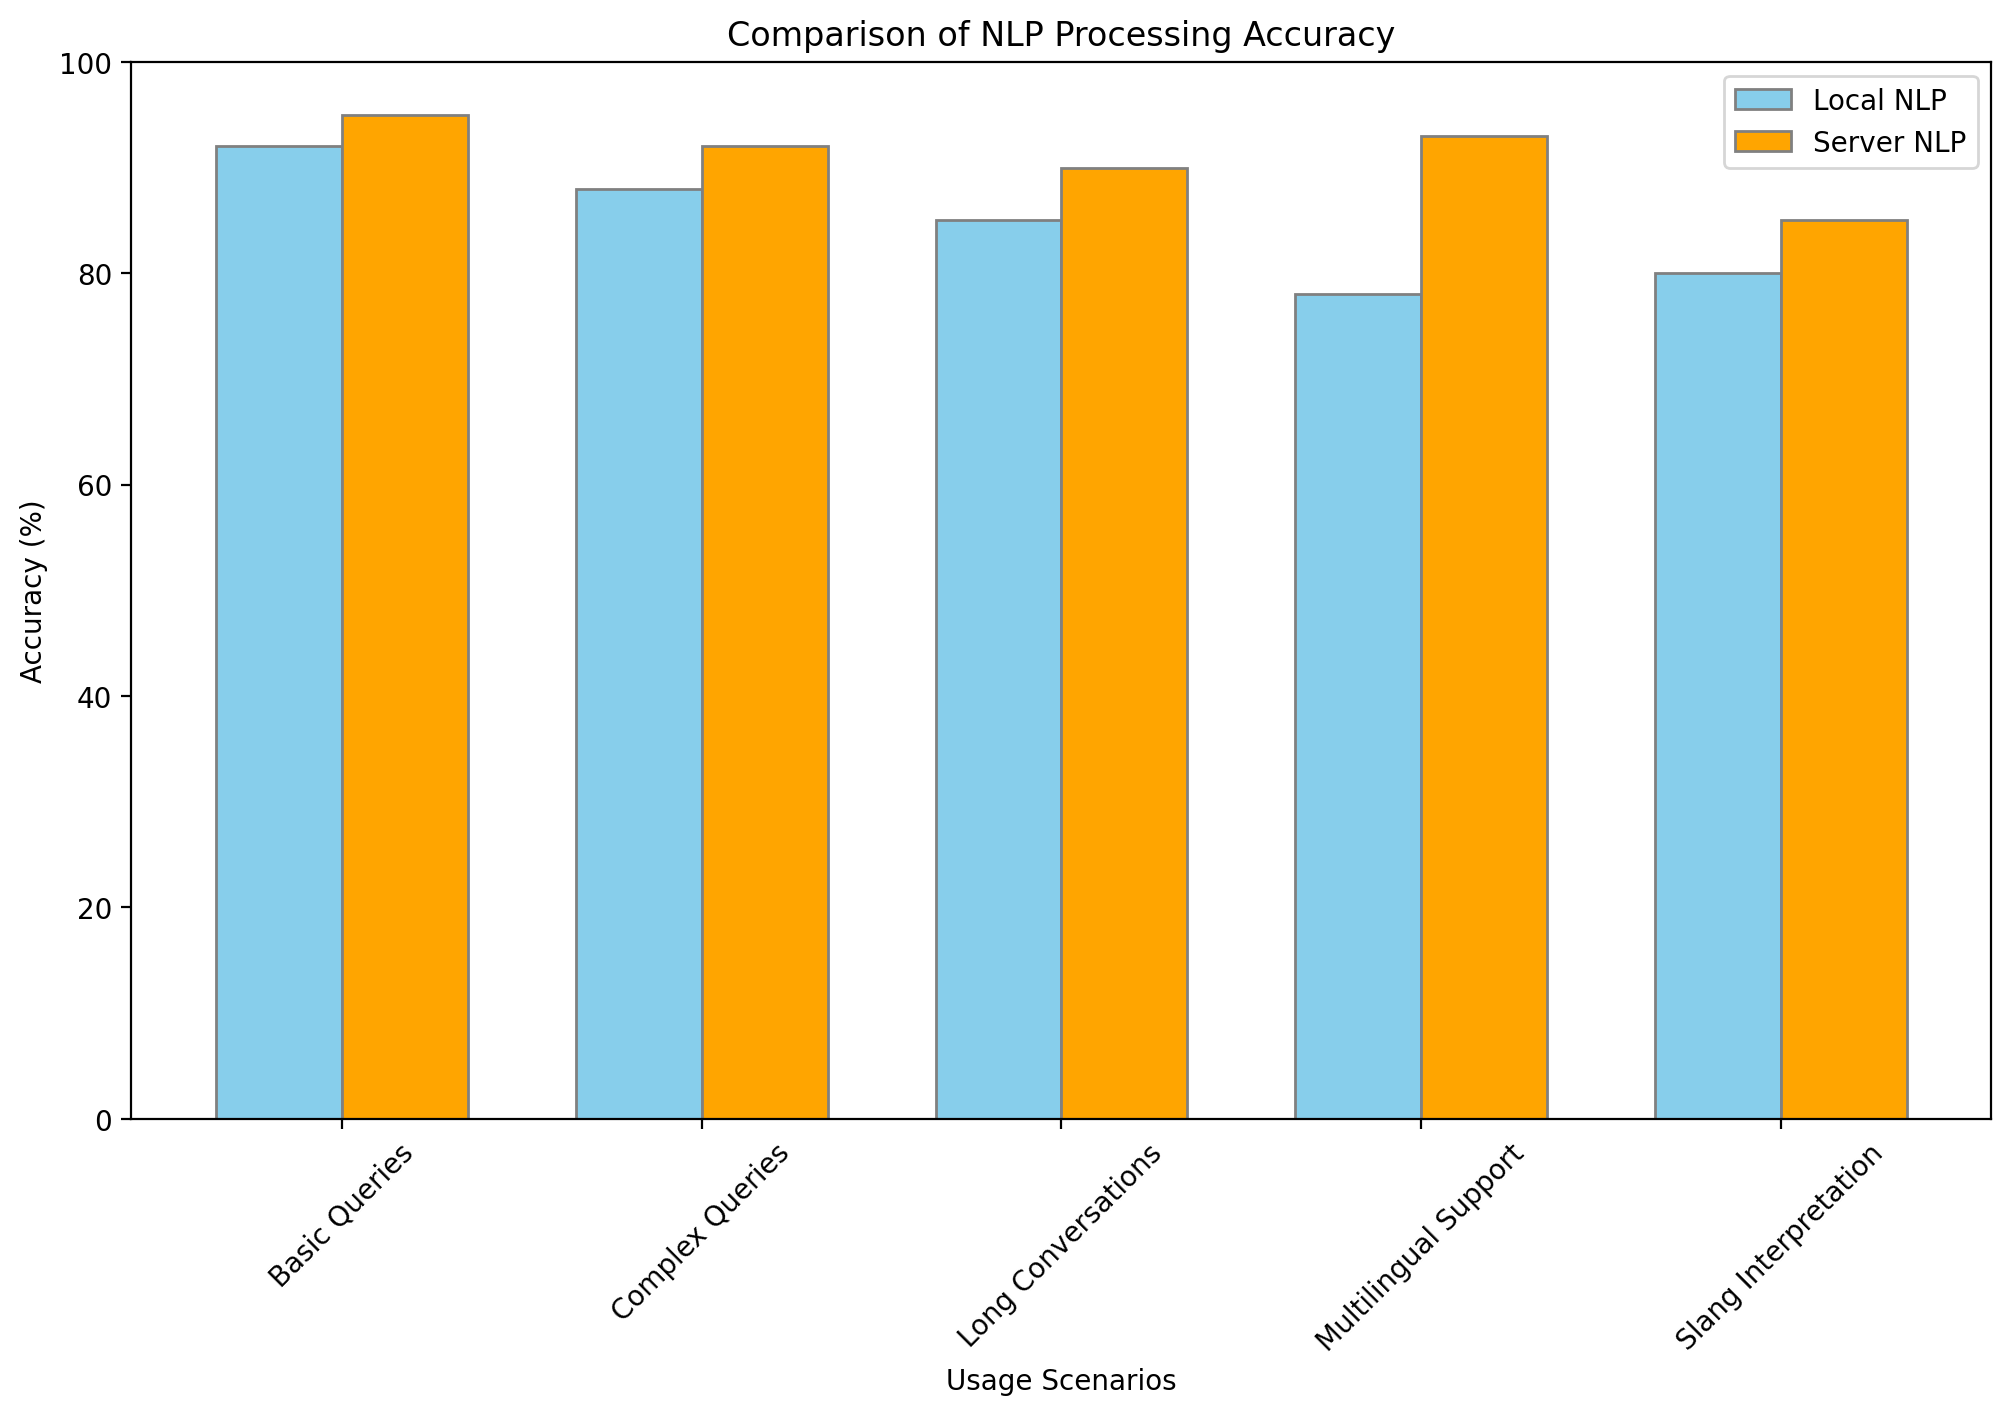
\includegraphics[width=0.8\linewidth]{nlp_correctness_graph.png}
    \caption{Mogelijke grafiek die correctheid van lokale NLP-verwerking vergelijkt met externe serverafhankelijke benaderingen. De x-as vertegenwoordigt verschillende gebruiksscenario's, terwijl de y-as de nauwkeurigheid aangeeft als een percentage.}
    \label{fig:nlp_correctness}
\end{figure}

Figuur \ref{fig:nlp_correctness} visualiseert de vermoedelijke prestatievoordelen van het privacybewuste toetsenbord in termen van NLP-verwerkingscorrectheid. De variatie in nauwkeurigheid onder verschillende scenario's biedt inzicht in de potentieel gunstige aspecten van de lokale verwerking.

\subsubsection{Gebruikersfeedback Over Pri\-va\-cy\-be\-sch\-er\-mende Functies}

\begin{figure}[ht]
    \centering
    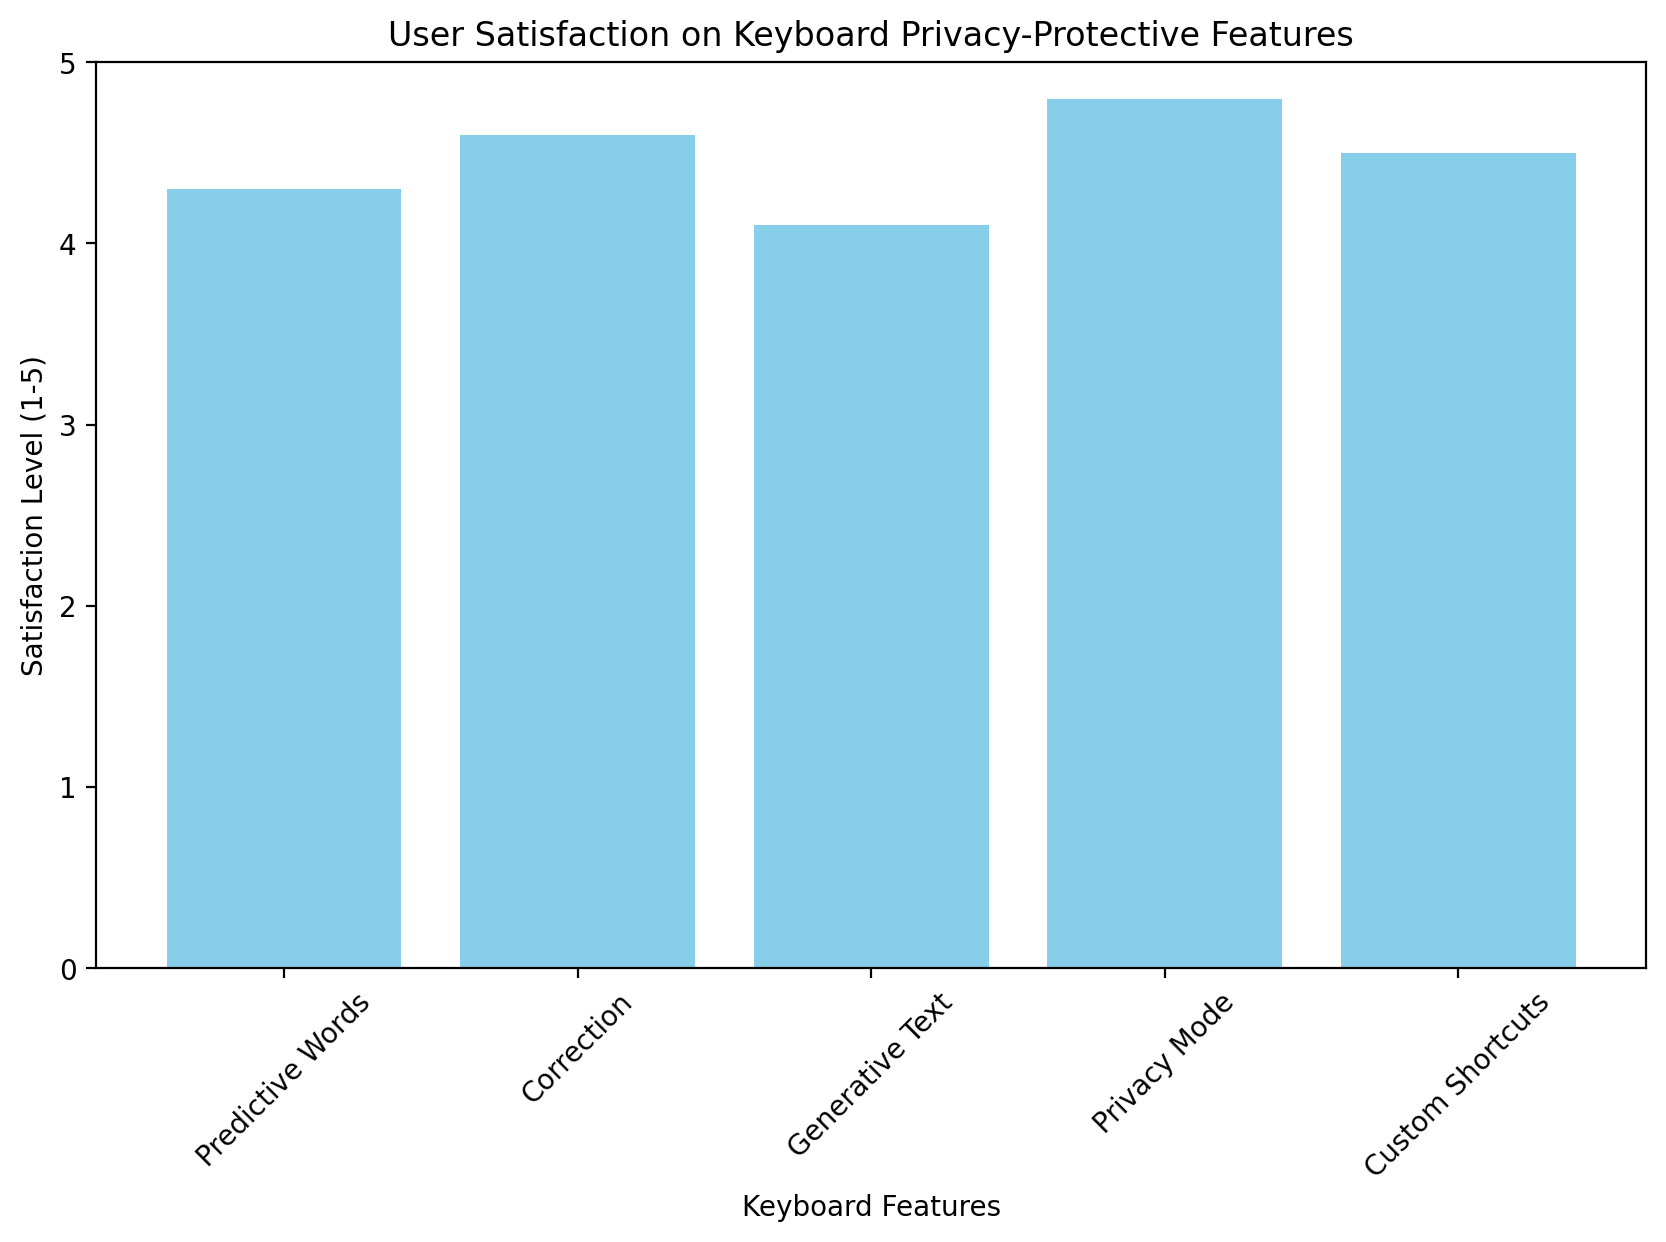
\includegraphics[width=0.8\linewidth]{user_feedback_chart.png}
    \caption{Mogelijke staafdiagram van gebruikersfeedback over toetsenbord functies. De x-as geeft verschillende functies weer, terwijl de y-as de mate van tevredenheid aangeeft op een schaal van 1 tot 5.}
    \label{fig:user_feedback}
\end{figure}

Figuur \ref{fig:user_feedback} presenteert de te verwachten reacties van gebruikers op toetsenbord functies. Door de mate van tevredenheid per functie visueel weer te geven, wordt duidelijk welke aspecten het meest gewaardeerd worden door de doelgroep.

\subsection{Conclusie}

De conclusie zal gebaseerd zijn op de vastgestelde resultaten en zal antwoord geven op de initiële onderzoeksvragen. Eventuele afwijkingen tussen de verwachte en daadwerkelijke resultaten zullen worden besproken, waarbij de impact op het vakgebied wordt belicht. Het succesvol creëren van het prototype is van cruciaal belang voor het behalen van de verwachte resultaten. Deze sectie zal de meerwaarde van de bachelorproef benadrukken door zowel technologische implementatie als gebruikerservaring in overweging te nemen.
